%% =============================================================================
%% THE SOFTWARE: PROMPT2ANALYTICS
%% =============================================================================

\section[The software: prompt2analytics (p2a)]{The software: \pkg{prompt2analytics} (\pkg{p2a})} \label{sec:tools}

\pkg{prompt2analytics} implements the three principles defined in
Section~\ref{sec:defining}. This section describes the software
architecture, the implemented methods, and the communication flow that
connects natural language requests to statistical computation.

\subsection{Architecture}

The software is organized as a \proglang{Rust} workspace with four
crates (Figure~\ref{fig:architecture}).

The core analytics library, \pkg{p2a-core}, implements all
statistical methods in pure \proglang{Rust} with no external
econometrics dependencies; all estimators are implemented from first
principles using \pkg{ndarray} for matrix operations and \pkg{faer}
for numerically stable linear algebra. The methods implemented are standard econometric procedures as
described in \citet{Wooldridge:2010} and
\citet{Cameron+Trivedi:2005} for regression and robust standard
errors, \citet{Baltagi:2013} for panel data,
\citet{Hamilton:1994} for time series, and \citet{Greene:2018} for
maximum likelihood estimation of discrete choice models. An optional
\code{cuda} feature flag enables GPU acceleration for
compute-intensive operations on NVIDIA hardware
(Section~\ref{sec:deployment}). Three user-facing crates provide
different access paths: \pkg{p2a-cli} produces a standalone
\code{p2a} binary with hierarchical subcommands organized by
analytical domain; \pkg{p2a-mcp} runs a Model Context Protocol server
exposing tools for LLM integration via stdio, HTTP, or WebSocket
transports; and \pkg{p2a-dioxus} provides a cross-platform graphical interface
using Dioxus~\citep{Dioxus}, a \proglang{Rust} framework that
compiles to WebAssembly for browser deployment, native desktop
applications, and mobile targets from a single codebase. All three
depend on \pkg{p2a-core}, ensuring identical numerical results
regardless of the interface used.

\begin{figure}[htbp]
\centering
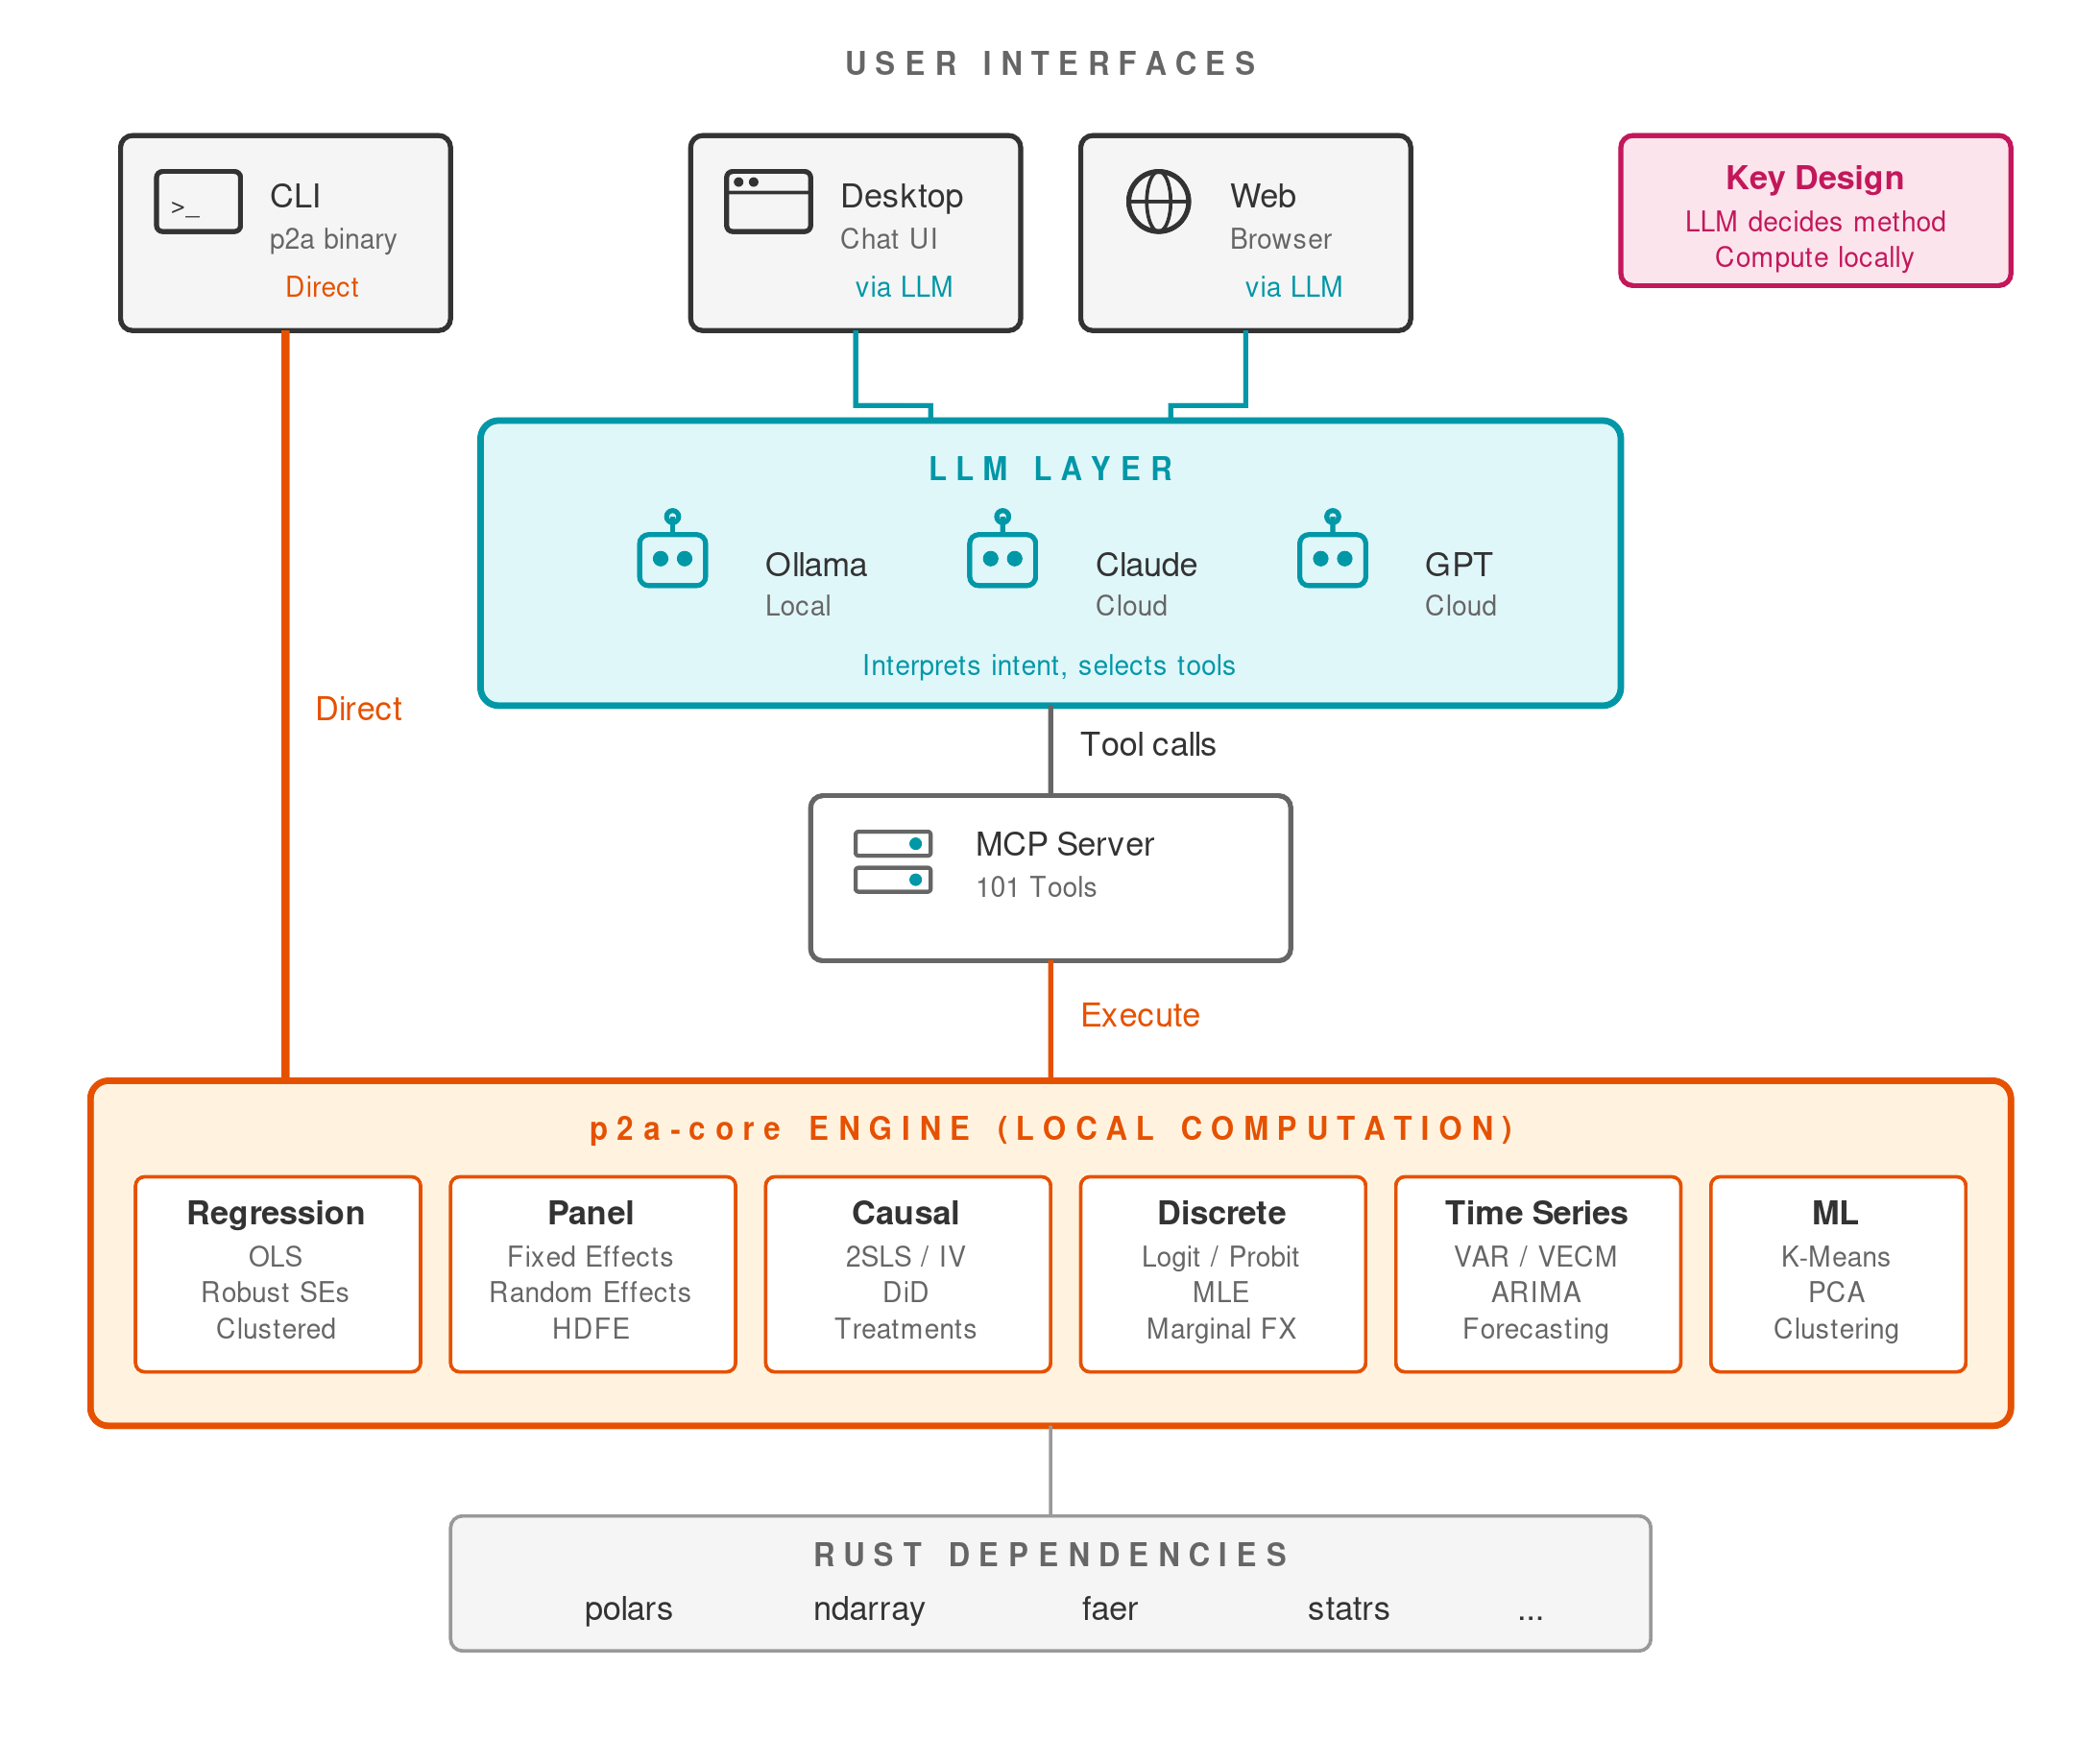
\includegraphics[width=\textwidth]{figures/architecture_v3}
\caption{Software architecture of \pkg{prompt2analytics}.
\textcircled{\raisebox{-0.5pt}{\scriptsize 1}}~Users interact via
terminal CLI, chat REPL, desktop app, or browser.
\textcircled{\raisebox{-0.5pt}{\scriptsize 2}}~An LLM interprets
the request and selects tools via the MCP server.
\textcircled{\raisebox{-0.5pt}{\scriptsize 3}}~All computation
executes locally in \pkg{p2a-core}; the CLI also accesses the
engine directly (orange path).}
\label{fig:architecture}
\end{figure}

The primary interface is conversational. Through the Dioxus web or
desktop application---or any MCP-compatible client such as Claude
Desktop---a user types:

\begin{Sinput}
User: Load wages.csv and regress salary on education and experience
      with robust standard errors.
\end{Sinput}

\noindent The language model interprets this request, selects the
appropriate tool (\code{regression\_ols} with \code{robust="hc1"}),
and returns both the numerical results and a natural language summary.
For scripting and automation, the same methods are accessible through
the CLI:

\begin{Sinput}
p2a data load wages.csv --name wages
p2a reg ols wages -y salary -x education experience --robust hc1
\end{Sinput}

\noindent Both pathways invoke the same \proglang{Rust} implementation
and produce identical numerical results.

\subsection{How the principles work in practice}

The communication flow (Figure~\ref{fig:chat-flow}) shows how
Principle~1 (separation) operates concretely:

\begin{enumerate}
  \item The user submits a natural language query.
  \item The LLM interprets the request and generates a structured tool
    call with parameters---e.g., \code{regression\_ols} with
    \code{y\_var="salary"}, \code{robust="hc1"}, and the relevant
    column names.
  \item The MCP server routes the call to the corresponding
    \proglang{Rust} method in \pkg{p2a-core}.
  \item The core library performs computation locally.
  \item Results (coefficients, standard errors, test statistics) are
    serialized to JSON and returned through the MCP server.
  \item The LLM receives the results and formulates a natural language
    explanation.
\end{enumerate}

\begin{figure}[htbp]
\centering
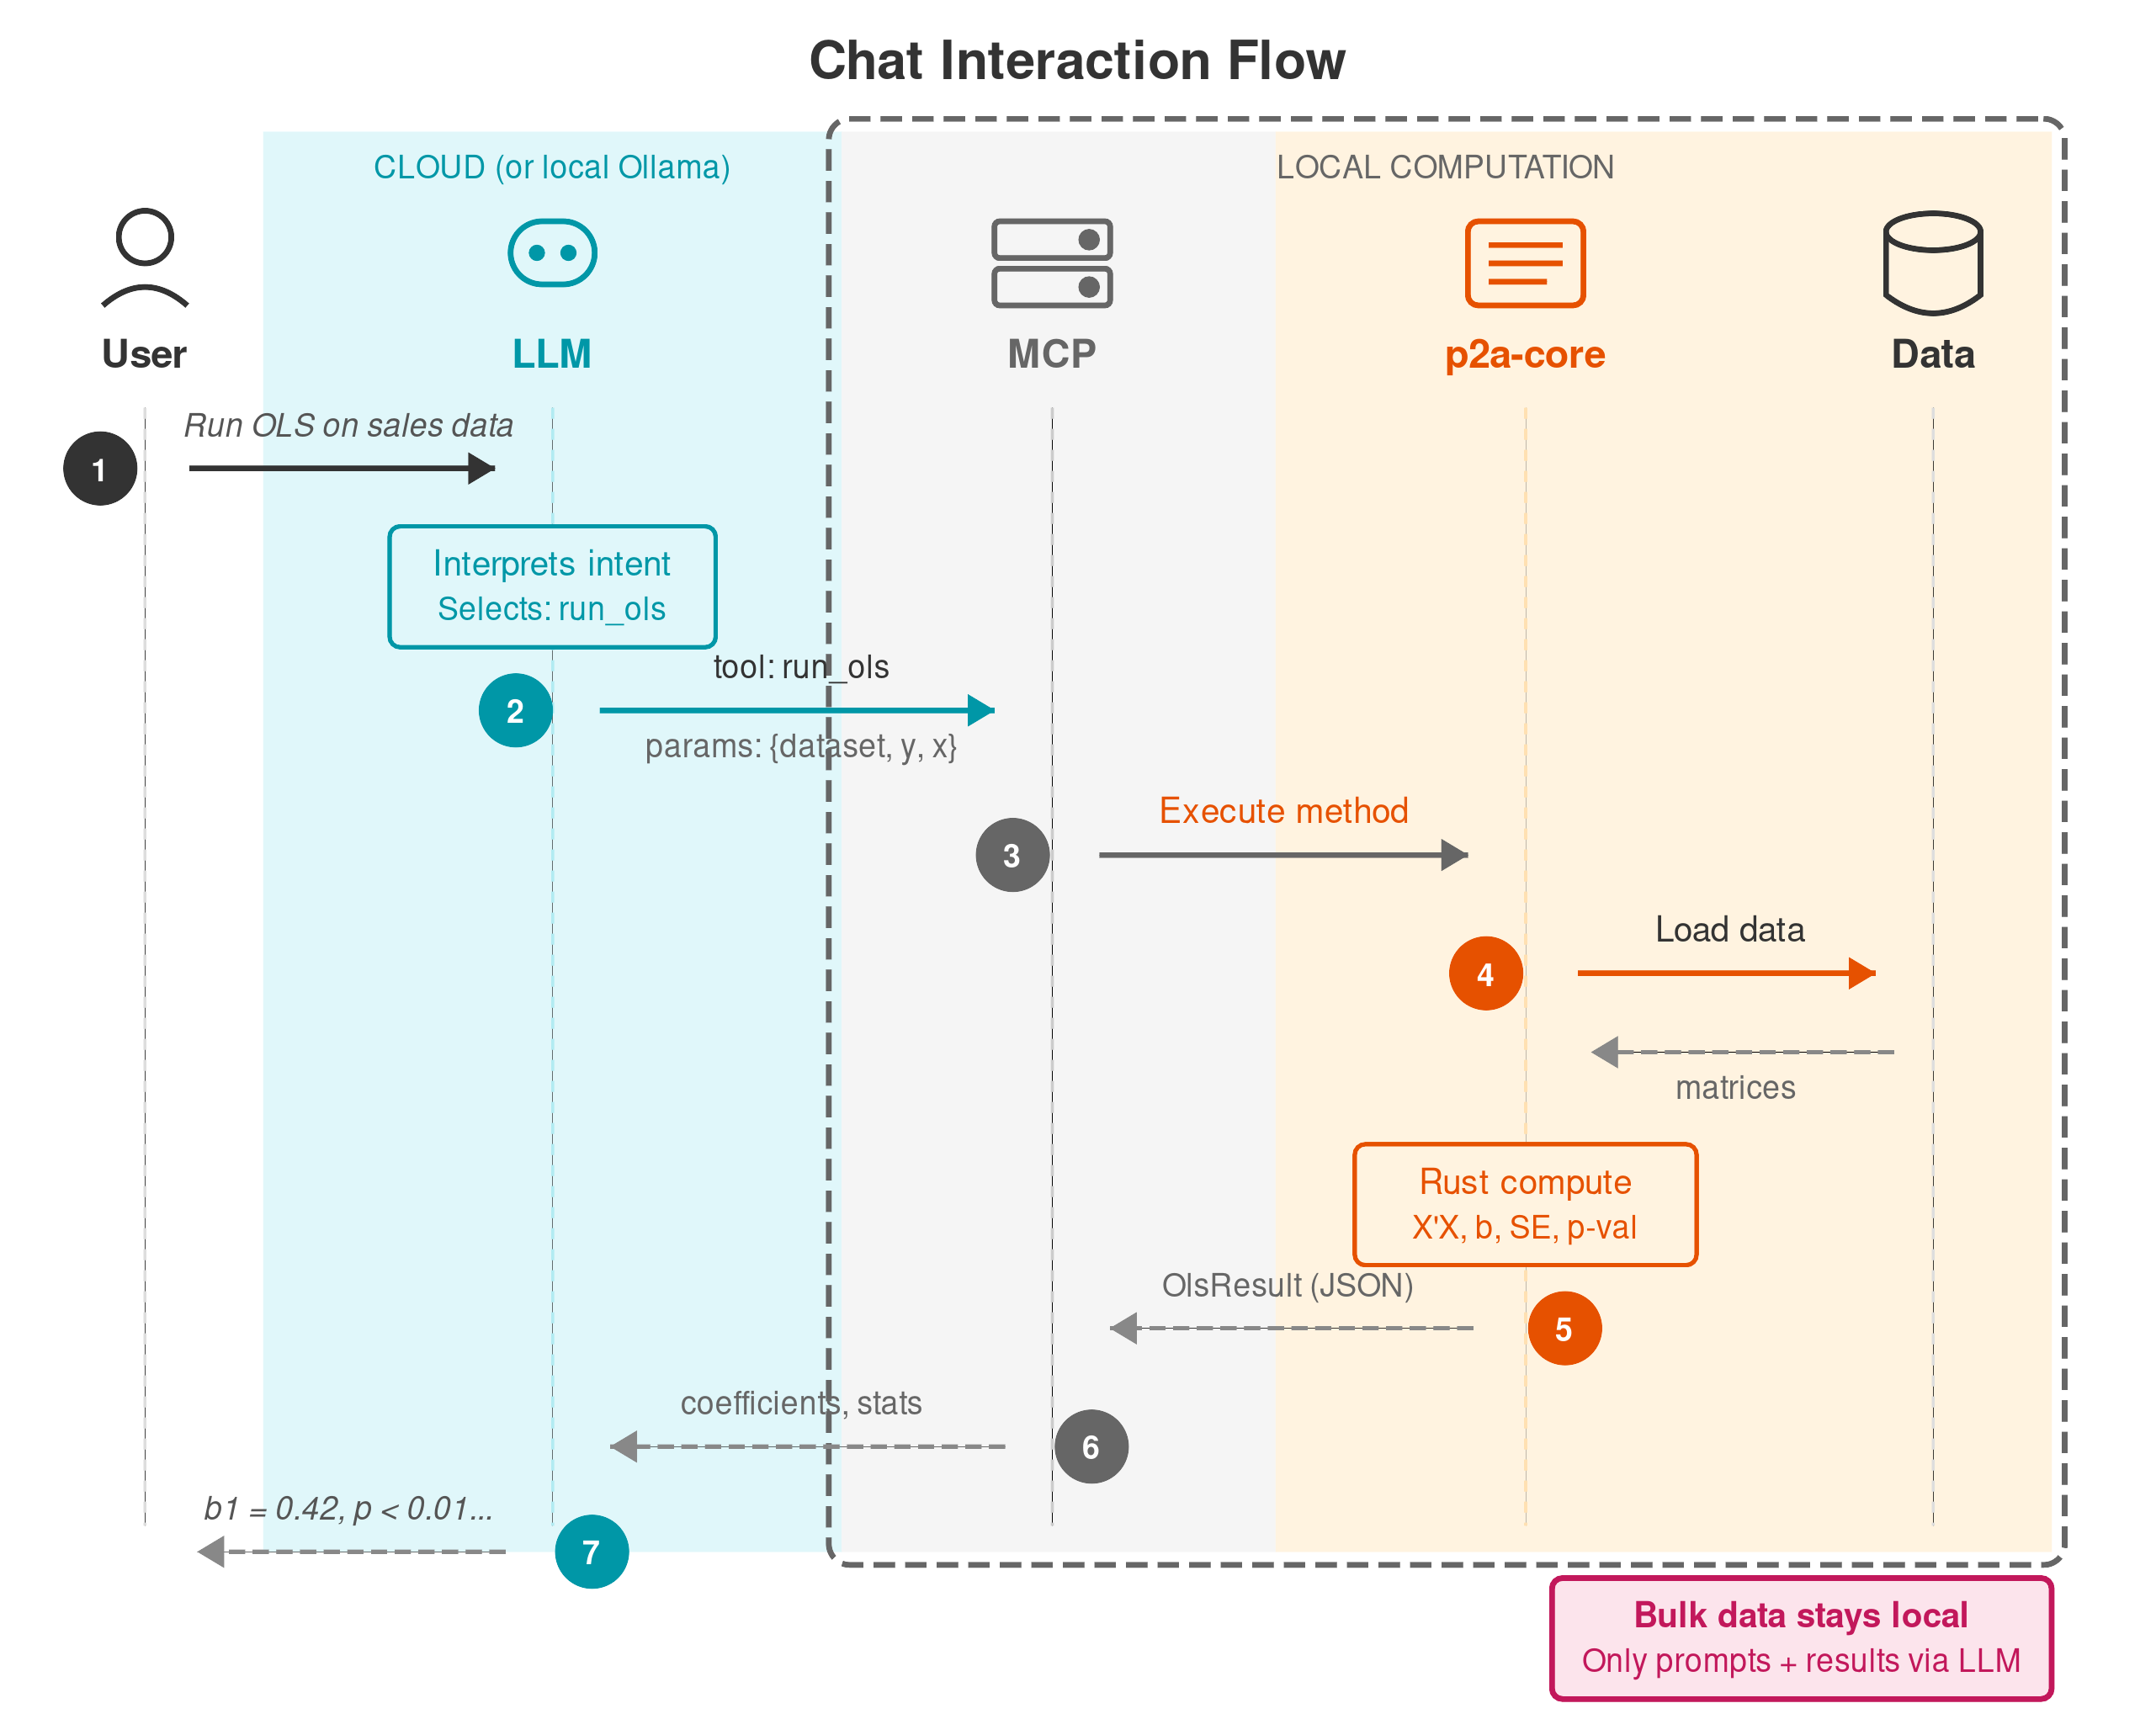
\includegraphics[width=\textwidth]{figures/chat_flow_v2}
\caption{Interaction flow from user request to result.
\textcircled{\raisebox{-0.5pt}{\scriptsize 1}}~The user describes
an analysis in natural language.
\textcircled{\raisebox{-0.5pt}{\scriptsize 2}}~The LLM interprets
the intent and emits a structured tool call with parameters.
\textcircled{\raisebox{-0.5pt}{\scriptsize 3}}~The MCP server
dispatches to the \proglang{Rust} engine.
\textcircled{\raisebox{-0.5pt}{\scriptsize 4}}~Data is loaded
locally into matrices.
\textcircled{\raisebox{-0.5pt}{\scriptsize 5}}~Results (JSON)
flow back through the MCP server.
\textcircled{\raisebox{-0.5pt}{\scriptsize 6}}--\textcircled{\raisebox{-0.5pt}{\scriptsize 7}}~The
LLM formats and explains the output to the user.
Bulk data (shaded region) never leaves the local machine.}
\label{fig:chat-flow}
\end{figure}

\noindent The LLM never sees raw data. It receives metadata at dataset
load time (column names, types, row counts) and aggregated results after
computation. Data preview tools (\code{head}, \code{sample}) do transmit
a small number of sample rows (default: 5 for \code{head}); for complete
data privacy, local LLM deployment via Ollama eliminates all external
transmission.

Each tool returns its full result as serialized text: for regression
this includes coefficients, standard errors, test statistics,
$R^2$, $F$-statistic, and information criteria (AIC, BIC); for
discrete choice, log-likelihood and pseudo-$R^2$; for time series,
parameter estimates and residual diagnostics. The LLM receives all
of these and decides what to present based on the conversational
context---typically highlighting coefficients and significance for a
first pass, and surfacing fit measures or diagnostics when the user
asks follow-up questions or when values are anomalous.

Each tool invokes a fixed, validated \proglang{Rust} function
(Section~\ref{sec:evaluation}). For linear regression, a
\code{LinearEstimator} trait provides a consistent interface:

\begin{Code}
pub trait LinearEstimator {
    fn coefficients(&self) -> &Array1<f64>;
    fn std_errors(&self) -> &Array1<f64>;
    fn t_values(&self) -> Array1<f64>;    // default impl
    fn p_values(&self) -> Array1<f64>;    // default impl
    fn residuals(&self) -> Array1<f64>;
    fn n_obs(&self) -> usize;
    fn df(&self) -> usize;
}
\end{Code}

\noindent Implementors provide core results (coefficients, standard
errors, residuals); derived statistics ($t$-values, $p$-values,
confidence intervals) are computed by default implementations, enforced
at compile time. The \code{LinearEstimator} trait currently covers OLS;
other model families use their own result types: discrete choice models
(\code{DiscreteResult}) return $z$-statistics, log-likelihood, and
pseudo-$R^2$; panel models (\code{PanelResult}) include $R^2$
(within for FE, overall for RE) and group structure; time
series models return information criteria and forecast output;
clustering methods return cluster assignments,
centroids, and inertia; and survival models use separate result types
for Kaplan-Meier curves, Cox regression (with hazard ratios), and
log-rank tests. All result types implement a common serialization
interface so the MCP layer can return structured output regardless of
the method family. Unlike, for example, \proglang{R}'s
formula interface, the API uses explicit column names---the natural
output of LLM parameter extraction, which identifies individual
columns rather than constructing formula syntax. This design also
simplifies the implementation: formula parsing, factor expansion, and
interaction term handling are unnecessary when the caller specifies
columns directly.

The \code{EconError} type provides structured error information
(singular matrix, convergence failure, insufficient clusters) that
enables the LLM to offer actionable recovery guidance.

Validation uses automated test suites that compare \proglang{Rust}
output against reference \proglang{R} packages on shared datasets.
Coefficients, standard errors, and test statistics are verified to
tolerances between $10^{-4}$ and $10^{-8}$ depending on the method.
When intentional differences exist---for example, using HC1 as the
default robust standard error estimator (rather than HC3), following
\proglang{Stata}'s convention---these are documented and tested
separately. The validation
approach is described further in Section~\ref{sec:evaluation};
Appendix~\ref{app:implementation} lists method-specific caveats and
known differences.

\subsection[Implemented methods (p2a-core)]{Implemented methods (\pkg{p2a-core})}

The \pkg{p2a-core} library implements over 200 statistical and
econometric methods, exposed as MCP tools.
Table~\ref{tab:method-categories} summarizes coverage, using standard
abbreviations: heteroskedasticity and autocorrelation consistent (HAC),
generalized least squares (GLS), high-dimensional fixed effects (HDFE),
two-stage least squares (2SLS).
Appendix~\ref{app:implementation} provides full documentation.

\begin{table}[htbp]
\centering
\begin{threeparttable}
\caption{Implemented method categories}
\label{tab:method-categories}
\small
\begin{tabular}{lp{9.5cm}}
\toprule
Category & Methods \\
\midrule
Regression & OLS with HC0--HC3, clustered SEs, HAC, bootstrap, GLS, NLS, LOESS, splines, stepwise, quantile regression \\
Panel data & FE, RE, Hausman, HDFE~\citep{Gaure:2013}, panel GLS, Arellano-Bond GMM, panel unit root tests (LLC, IPS, Fisher) \\
IV & 2SLS, first-stage diagnostics, Sargan test, GMM \\
Causal (design) & DiD, staggered DiD~\citep{Callaway+SantAnna:2021}, Bacon decomposition~\citep{Goodman-Bacon:2021}, ETWFE~\citep{Wooldridge:2025}, sharp/fuzzy RD with CCT~\citep{Calonico+etal:2014}, multi-cutoff RD, synthetic control~\citep{Abadie+etal:2010}, gsynth~\citep{Xu:2017}, SCPI~\citep{Cattaneo+etal:2021} \\
Causal (treatment) & IPW, AIPW, matching, CBPS~\citep{Imai+Ratkovic:2014}, entropy balancing, GBM weighting, TMLE~\citep{vanderLaan+Rose:2011}, CTMLE, LTMLE, DML~\citep{Chernozhukov+etal:2018} \\
Discrete choice & Logit, probit, multinomial, conditional, mixed, ordered, negative binomial, ZIP/ZINB, hurdle \\
Time series & ARIMA, VAR, VARMA, VECM, IRF, Granger causality, STL/MSTL, Holt-Winters, structural TS, Kalman filter, GARCH, changepoint \\
Spatial & SAR, SEM, SAC, spatial probit, spatial panel, spatial GMM \\
Survival & Kaplan-Meier, log-rank, Cox PH, AFT, competing risks \\
Mediation & Causal mediation, natural effects, sensitivity~\citep{Cinelli+Hazlett:2020}, E-values, Balke-Pearl bounds \\
Statistical tests & 50+ tests: $t$-tests, ANOVA, MANOVA, $\chi^2$, Fisher, Wilcoxon, Kruskal-Wallis, Friedman, Shapiro-Wilk, KS, Tukey HSD \\
\bottomrule
\end{tabular}
\begin{tablenotes}[flushleft]
\item \emph{Note:} Appendix~\ref{app:implementation} provides full
documentation. Table~\ref{tab:method-coverage} lists unimplemented
categories with recommended alternatives.
\end{tablenotes}
\end{threeparttable}
\end{table}

\subsection[The MCP tool layer (p2a-mcp)]{The MCP tool layer (\pkg{p2a-mcp})}

The \pkg{p2a-mcp} server exposes tools organized into categories that
mirror the core library (Table~\ref{tab:mcp-tools}).

\begin{table}[htbp]
\centering
\begin{threeparttable}
\caption{MCP tool categories}
\label{tab:mcp-tools}
\small
\begin{tabular}{llr}
\toprule
Category & Examples & Tools \\
\midrule
Data management & \code{load\_dataset}, \code{describe\_dataset} & 7 \\
Data transformation & \code{munge\_filter}, \code{munge\_join}, \code{munge\_pivot} & 19 \\
Regression & \code{regression\_ols}, \code{regression\_diagnostics} & 10 \\
Panel data & \code{panel\_fixed\_effects}, \code{hausman\_test} & 5 \\
Causal inference & \code{iv\_2sls}, \code{diff\_in\_diff} & 8 \\
Discrete choice & \code{logit}, \code{probit} & 2 \\
Time series & \code{ts\_arima\_fit}, \code{ts\_var} & 6 \\
Statistics & various hypothesis tests & 30+ \\
Visualization & \code{viz\_scatter}, \code{viz\_histogram\_interactive} & 7 \\
\bottomrule
\end{tabular}
\begin{tablenotes}[flushleft]
\item \emph{Note:} Tool count per category. Each tool corresponds to
one or more \pkg{p2a-core} methods and is described by a JSON Schema
that LLMs use for parameter extraction.
\end{tablenotes}
\end{threeparttable}
\end{table}

Each tool has a JSON Schema defining required and optional parameters.
Schema design minimizes required parameters to reduce LLM errors and
provides sensible defaults (e.g., HC1 for robust standard errors).
Tool descriptions are written to be interpretable by LLMs, specifying
when each tool is appropriate. For example:

\begin{verbatim}
{
  "name": "regression_ols",
  "description": "Run OLS regression with optional robust SEs",
  "inputSchema": {
    "required": ["dataset", "y_var", "x_vars"],
    "properties": {
      "dataset": {"type": "string"},
      "y_var": {"type": "string"},
      "x_vars": {"type": "array", "items": {"type": "string"}},
      "robust": {"type": "string", "enum": ["hc0","hc1","hc2","hc3"]},
      "cluster_var": {"type": "string"}
    }
  }
}
\end{verbatim}

\noindent Note the distinction between MCP tools and core methods:
tools serve as entry points that may invoke multiple methods. The
\code{regression\_ols} tool provides access to OLS with several
covariance estimators (HC0--HC3, clustered, HAC), each a distinct
method in \pkg{p2a-core}. This many-to-one mapping keeps the LLM's
selection task manageable while preserving access to the full library.

After consolidation, the full MCP server exposes approximately
270~tools whose JSON schemas consume ${\approx}\,32{,}000$
tokens---a substantial share of current context windows.  Since
sending all schemas with every request would leave little room for
conversation history, the built-in chat interface filters to
119~Tier-1 tools (${\approx}\,20{,}000$ tokens), covering
the most common analytical workflows.  The evaluation in
Section~\ref{sec:evaluation} uses this same 119-tool set.
External MCP clients receive the complete schema and can apply
their own filtering.

\paragraph{Multi-turn context management.}
The token cost of tool schemas directly affects how many
conversational turns a model can sustain.  To manage this, the system
includes prior tool calls and their results in the conversation
history sent to the LLM.  Each assistant message that triggered a tool
call is preserved with its structured \code{tool\_calls} field,
followed by a \code{tool} role message containing the result
(truncated to 2{,}000 characters to prevent context overflow). This
enables the LLM to resolve references like ``those results'' or ``now
try with clustered standard errors'' by inspecting what was previously
computed.  A token budget tracker estimates context usage across the
system prompt, conversation history, tool schemas, and the current
query; when the budget approaches the model's context window, older
turns are summarized (retaining tool names and key results) while
recent turns are kept verbatim.  With the 119-tool schema, a
128K-context model supports roughly 25--35 substantive turns before
summarization begins.  External MCP clients (e.g., Claude Desktop,
Cursor) manage their own context windows and may apply different
truncation or tool-filtering strategies.

Beyond executing methods, the system generates data-driven warnings
when results suggest potential violations of identifying assumptions.
Warnings are non-blocking---results are always returned---but they highlight
conditions that warrant careful interpretation.

For instrumental variables, first-stage $F$-statistics are checked
against the Stock--Yogo threshold of 10~\citep{Stock+Yogo:2005}. For
staggered difference-in-differences, pre-trend tests are computed
automatically. For matching, balance diagnostics flag
standardized mean differences exceeding 0.1~\citep{Austin:2011}. For
regression discontinuity, effective sample sizes within the bandwidth
are checked against minimum thresholds.

Each warning includes a severity level, a diagnostic message,
the assumption at risk, and suggested remediation steps. This
structured information enables the LLM to provide recovery guidance
rather than generic failure messages. The thresholds are
deliberately conservative (e.g., $F < 10$ for weak instruments,
SMD $> 0.1$ for balance), which may produce false positives in
settings where these rules of thumb are known to be overly
strict. We prefer occasional unnecessary warnings to missed
violations; users can evaluate the diagnostic evidence and
disregard warnings they judge inapplicable.

\subsection{Implementation choices}

The choice of \proglang{Rust} follows from two requirements:
validated methods must remain correct across deployments, and the
analytics engine must run efficiently on the user's own machine.
In a chat-first architecture, users interact through natural language
rather than writing code in \proglang{R} or \proglang{Python}---so the
implementation language need not be one that researchers already know.
This frees the choice to optimize for technical properties:
\proglang{Rust}'s compile-time memory safety eliminates buffer
overflows, use-after-free, and data races that can cause incorrect
results in numerical software; its zero-cost abstractions and
fine-grained control over parallelism and memory layout deliver
compiled performance that lets the same engine run locally on the
user's machine rather than requiring cloud infrastructure.
A single codebase compiles to standalone binaries, WebAssembly for
browsers, and shared libraries for language integration.

The practical barrier to implementing well-established statistical
methods in a systems language has also fallen dramatically.  Agentic
coding tools and highly capable LLMs for code generation make it
feasible to produce high-quality, validated implementations of
textbook algorithms at low marginal cost---and this cost continues to
decline.\footnote{Nearly all \proglang{Rust} code in
\pkg{prompt2analytics} was written with the assistance of Claude Code
(Anthropic's agentic coding tool), including the core statistical
implementations, MCP server, and test suites.  Human review focused on
algorithmic correctness, API design, and validation against reference
implementations.}

The ecosystem provides the necessary components: \pkg{polars} for
data manipulation~\citep{polars}, \pkg{ndarray} for array operations,
and \pkg{faer} for linear algebra. All computations use 64-bit
floating-point arithmetic throughout, matching \proglang{R}'s precision. To
our knowledge, no econometrics or data analytics library has previously been available for \proglang{Rust};
\pkg{p2a-core} addresses this gap.

Several additional design choices merit brief explanation. For
conversation persistence, the web application uses SurrealDB, an
embedded document database for storing conversation history. Its
embedded operation requires no external service; its flexible schema
accommodates evolving conversation structures without migrations.
Analytical datasets are held in memory during sessions and not
persisted, limiting storage to lightweight metadata.

When users request methods outside the implemented set, the LLM
infers scope from the tool schema. In some cases, it maps to the
closest available alternative and explains the substitution; in
others it reports unavailability.

Regarding security, tools have fixed descriptions embedded in the
server binary---external modification requires rebuilding. No
arbitrary code execution is possible. Tool calls are logged and can be
inspected. Dataset access requires explicit loading; the server
has no ambient filesystem access. Nevertheless, users should avoid
loading untrusted data files that could contain injection payloads,
and prefer local LLM deployment for high-security environments.
